\chapter{Detecting corruption, collusion \& fraud: Data product}\label{chap_product}


This chapter first describes the details in the modeling process for the identification of possible cases of corruption, collusion and fraud within the World Bank's Major and Historical awards and investigations data. After that, this chapter explains  how does the visualization created for the World Bank's investigation team in the Integrity Vice Presidency works. Section \ref{sec_pipeline} is visualization of the data pipeline that sustains the web application that runs in the Wolrd Bank's servers. Section \ref{sec_models} gives the details of the model selected for the identification of corruption, collusion and fraud and finally, section \ref{sec_visual} shows the different visualizations made for a more proactive investigation process.

\section{Data pipeline} \label{sec_pipeline}

As chapter \ref{chap_data} shows, there are different data sources, figure \ref{fig_pipeline} shows a summary of how the data from all the sources was combined into a web application that runs in the server of the World Bank and helps the investigators at the Integrity Vice Presidency to investigate projects and entities in a more proactive way than by relying on whistle-blowers. Figure \ref{fig_pipeline} shows how the different data sources first combine into the Google Algorithm for name disambiguation explained on chapter \ref{chap_data}. Then the resulting tables are joined with the World Bank's Development indicators for each country. After this, all the country specific and co-award network features explained in section \ref{sec_features} were produced so that finally everything feeds the model that can potentially identify malicious contracts or contractors.

\begin{figure}[H]
\begin{center}
\caption{Data pipeline}
\label{fig_pipeline}
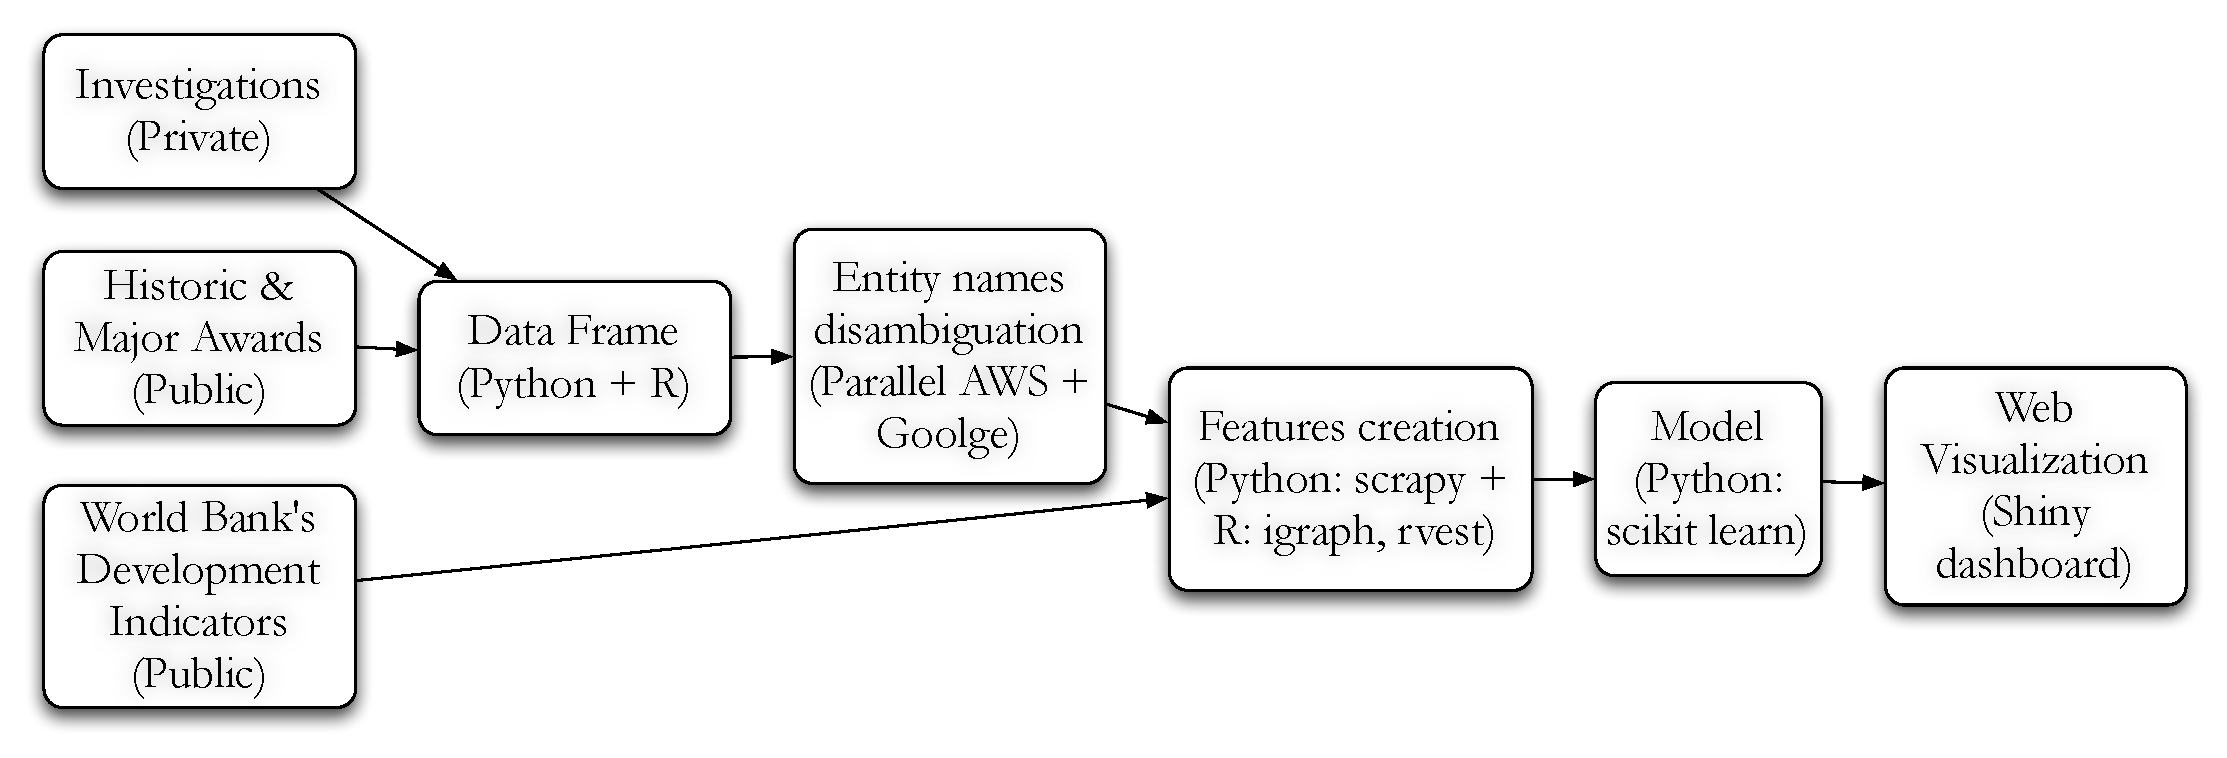
\includegraphics[width=\textwidth,height=1\textheight,keepaspectratio]{../img/pipeline.pdf}
\end{center}
\noindent \footnotesize{\textbf{Source:} Own creation.}
\end{figure}

The steps illustrated  in figure \ref{fig_pipeline} were explained in previous chapters up to the feature creation. The next sections cover the modeling and the visualizations.

\section{Model} \label{sec_models}

As the introduction says in page \pageref{dssg} any Data Science project such as this one requires a solvable problem, that is challenging, has impact, has relevant data and committed partner. Up to this face we have stated that detecting corruption, collusion and fraud  is challenging enough, the Google searches algorithm and the co-awards network is a clear example of that. The impact was stated in figures such as \ref{fig_major_awarded_usd} that shows the amount that the World Bank gives in its procurements contracts in its effort to reduce global poverty. It more than enough and relevant data  from different sources that complement to each other and a clearly committed partner. Up to this point the project is just missing a solution to identification of corruption, collusion and fraud such that it becomes a solvable problem.  

We needed to create a solvable problem within the time restrictions stated at the time of the project. Unfortunately, the most relevant data came way after the project started and the name disambiguation algorithm took long enough to have long enough time for the next steps of the project, which was, the modeling step. The idea is to find a model that is able to identify potential cases of corruption, collusion or fraud within the World Bank's data. 

A traditional modeling process like this involves comparing different approaches in order to minimize the desired error or maximize the accuracy of a classification or prediction.


For this project, three different models were considered, a classifier  using a Supported Vector Machine (SVM), a Random Forest and a Logistic Regression. To evaluate the output we created the dependent variable by considering the labels in the investigations data by labeling any substantiated case as guilty and not guilty in any other case. See \cite{hasti} for more details on SVM, random forest and logistic regression. 


To select the models first we took a training set from the data by sorting by date so that the data for the past would be able to identify potential corruption, collusion and fraud in the data for the future relative to the training data. To select the parameters of each model we used some crossed validation in terms of the Area Under Curve (AUC) of the Receiver Operating Characteristic curve (ROC), ROC-AUC. See \ref{chap_code} and the code \ref{code_models} to see how the parameters of the models were selected.

Since all the investigations data was private, unfortunately for this paper,  the modeling phase cannot be replicated because of the access to the data so the paper cannot show the results of the different models tunned. Nevertheless, after tunning with different parameters and considering different features, the resulting model was a Random Forest which has a ROC curve that can be seen at figure \ref{fig_roc}. The figure \ref{fig_roc} contains the percentage of the  investigated and not guilty contracts that were marked  by the model as ``should be investigated'' (false positive rate) against the percentage of investigated contracts caught by the model (true positive rate).The figure shows in green the ROC curve for the random forest considering the co-awards network features and the blue curve refers to the ROC without the co-awards network features. As it can be seen from the figure, the network features add accuracy to the prediction so they are very desirable for the World Bank Investigators.

It is also important to notice here that the random forest is a great model for the investigators at the Integrity Vice Presidency because it is a much better classifier than the actual benchmark which was just guessing whether they should investigate a contract, entity or project or not. The dashed line in figure \ref{fig_roc} represents a random guess, so the farther the ROC curve is from that line, the better the quality of the classification.

\begin{figure}[H]
\begin{center}
\caption{ROC: Random forest test data}
\label{fig_roc}
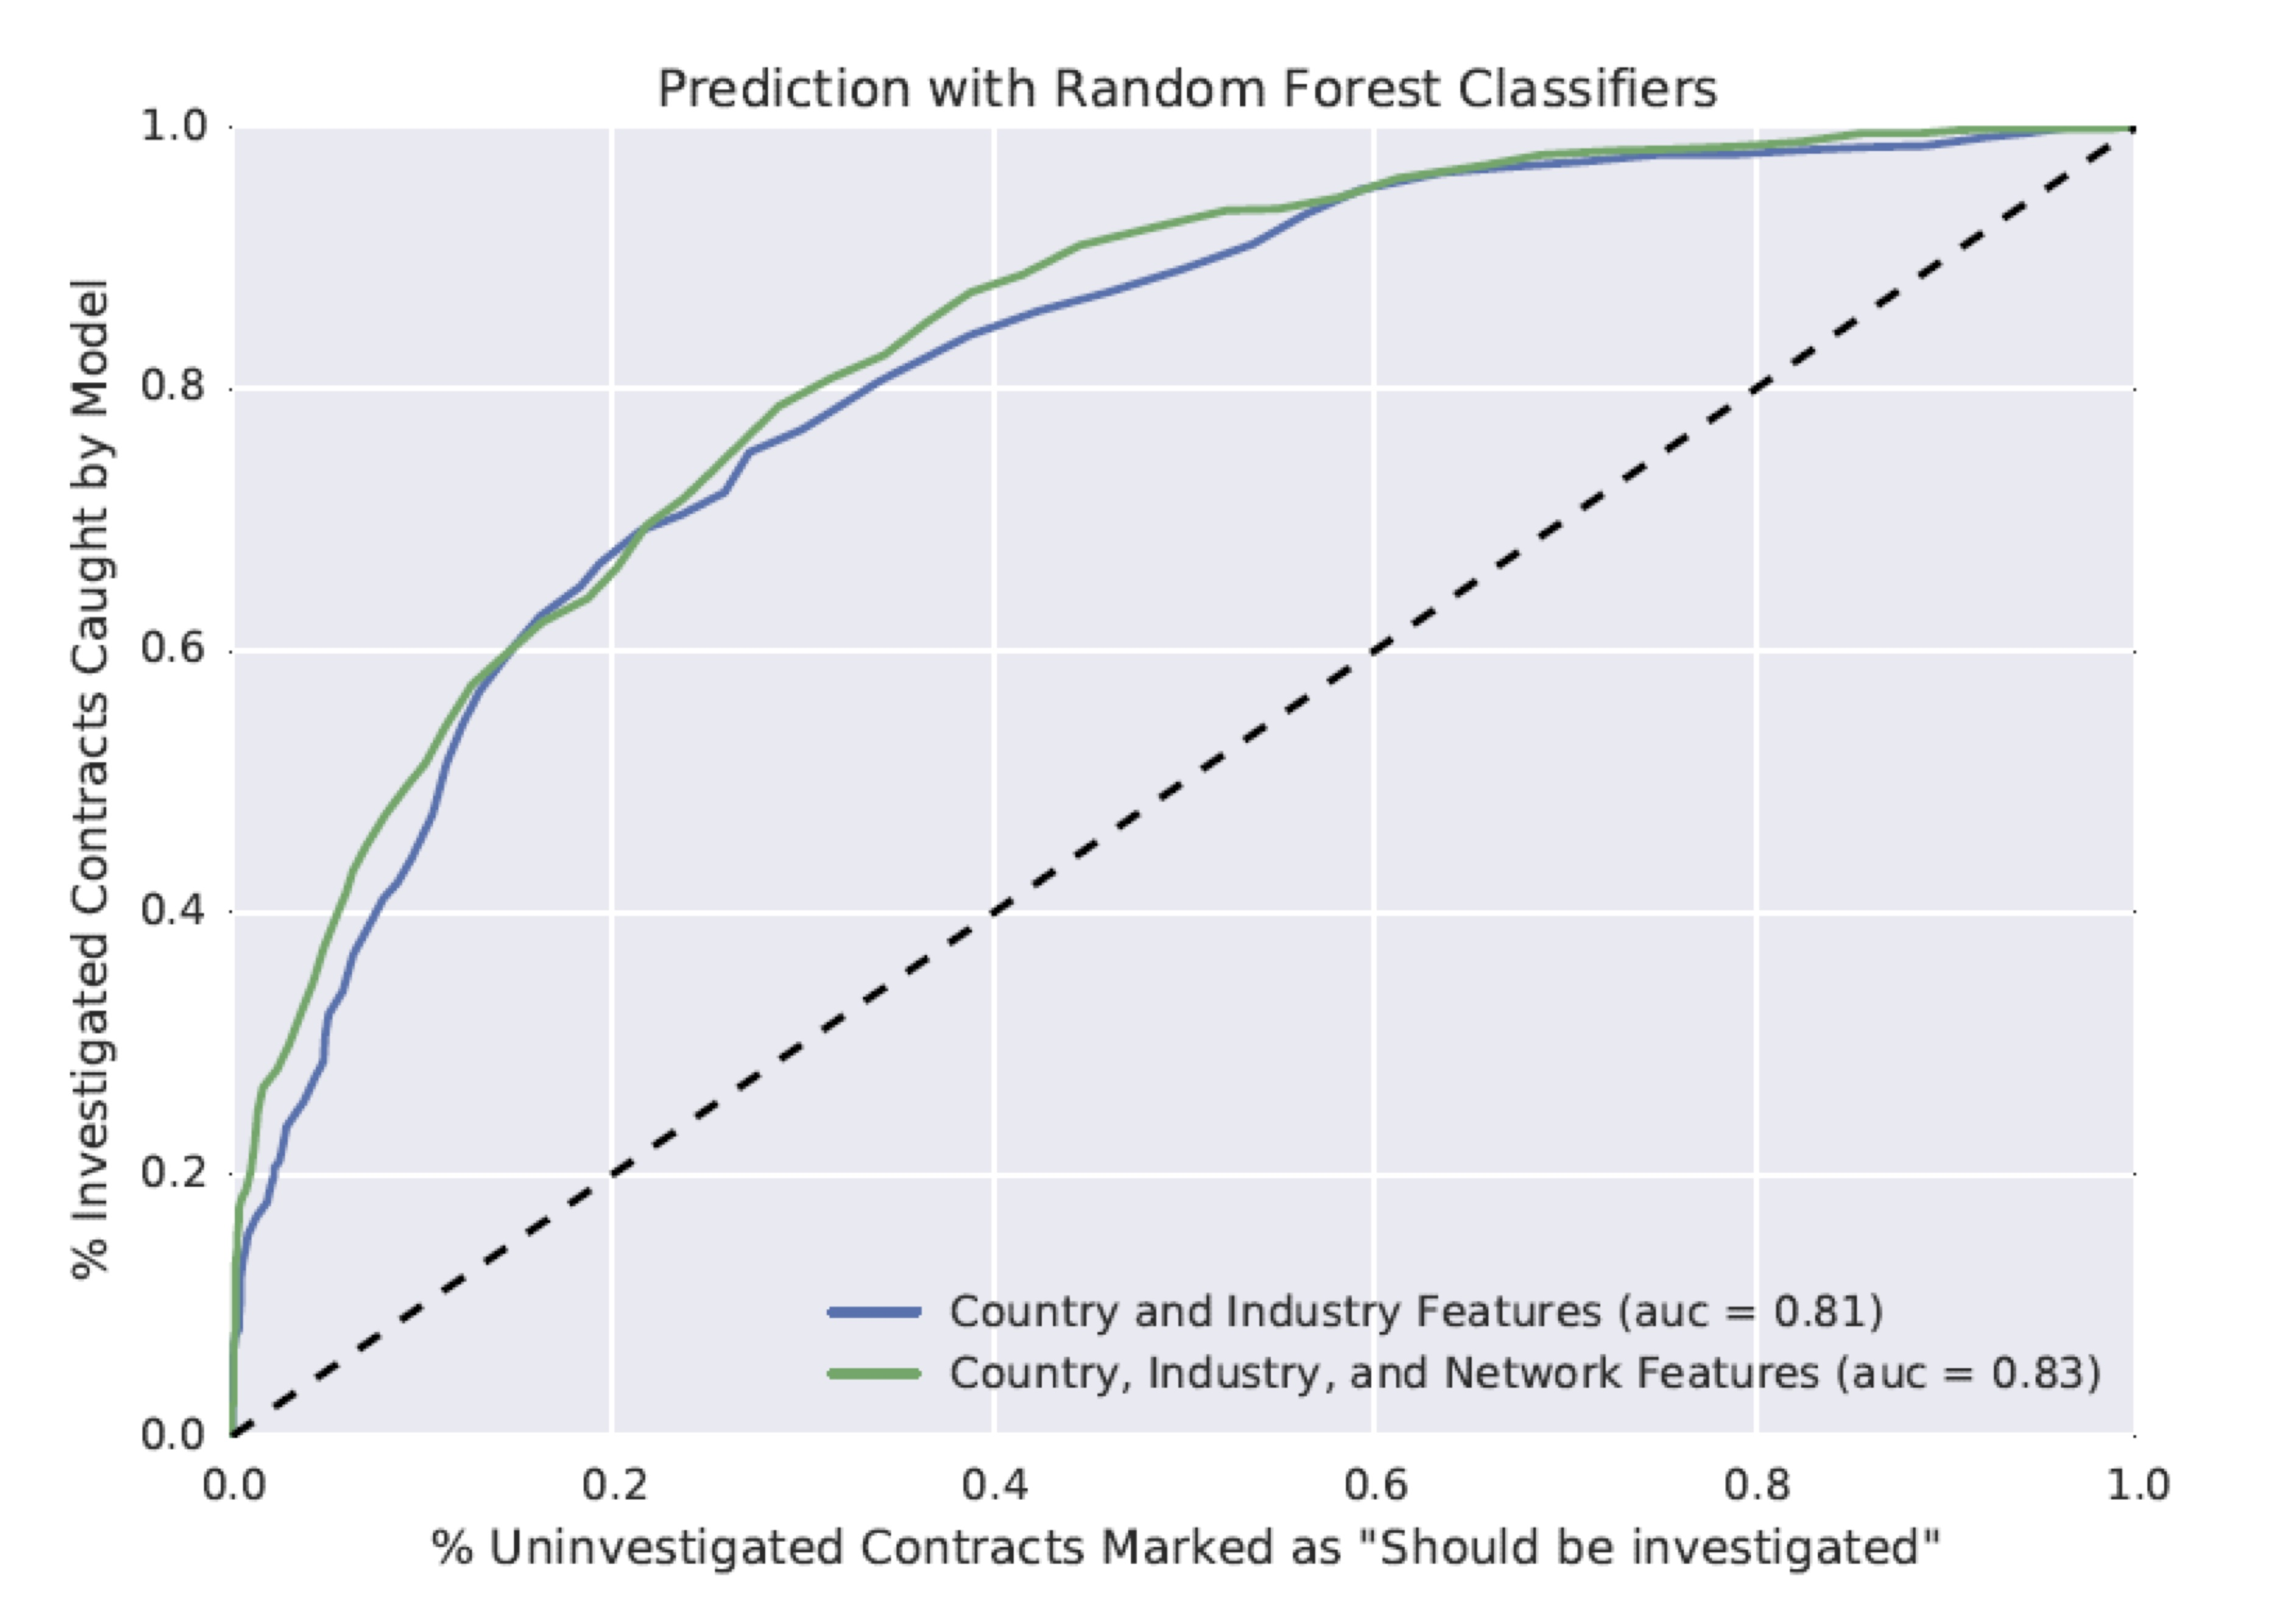
\includegraphics[width=1.05\textwidth,keepaspectratio]{../img/roc.jpg}
\end{center}
\noindent \footnotesize{\textbf{Source:} Own creation.}
\end{figure}


\section{Web visualization application: dashboard} \label{sec_visual}

In order for the investigators at the World Bank to look for suspicions patterns of corruption, collusion and fraud in their procurement data in a proactive way and not by waiting for whistle-blowers to alert them about potential  problems in the procurements process and, also, to use the classification model to target their investigations to the entities, projects and contracts that have higher risk of being a substantiated case if investigated, in this project we created a web application that helps them do their work.

\subsection{Dashboard outline}


\subsection{Red-flags from data}

Chapter \ref{chap_procurements} presented figure \ref{fig_what_corr} suggesting ideas of how to look for common patterns to identify potential cases of corruption, collusion, fraud, coercion and other types of malicious behavior among the procurements that the World Bank gives to countries all over the world. The objective of this section is to try to replicate those figures by using real data in order to provide a valuable insight to the investigators working in the Integrity Vice Presidency to help them attack this problem.

\subsection{Interactive map}

\begin{figure}[H]
\begin{center}
\caption{Interactive map}
\label{fig_interactive_map}
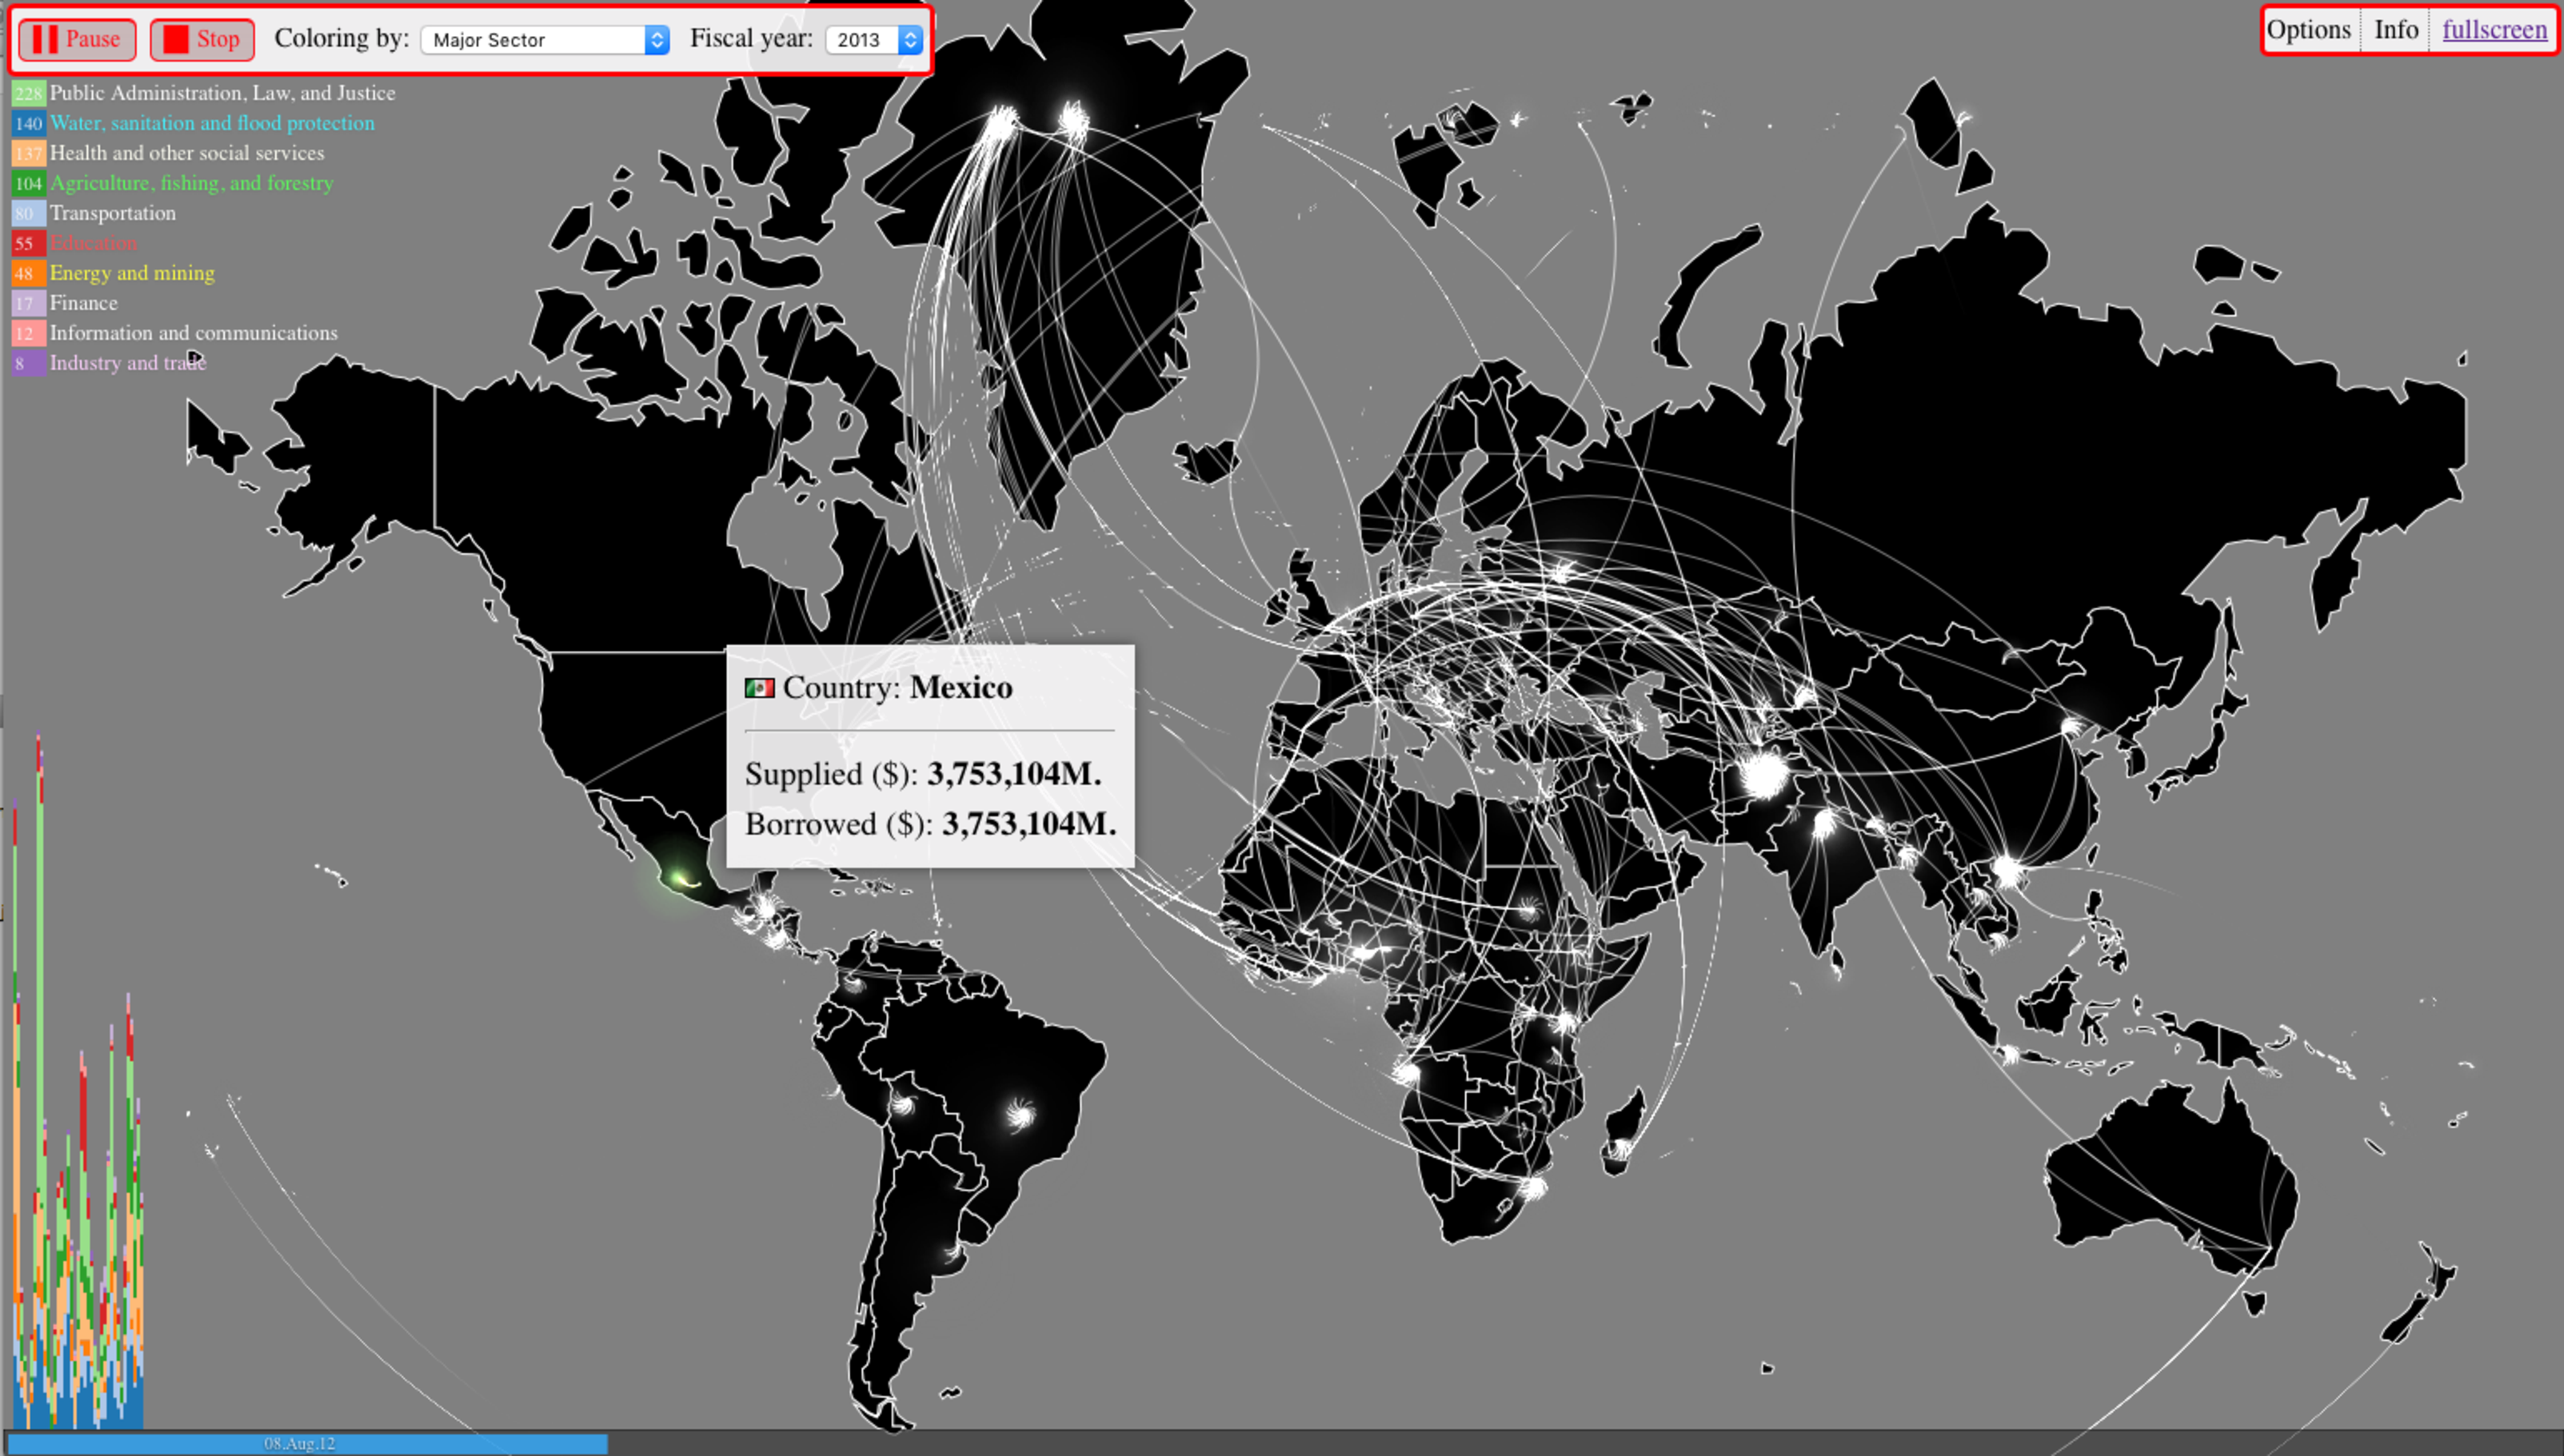
\includegraphics[width=\textwidth,height=1\textheight,keepaspectratio]{../img/interactive_map_mex.pdf}
\end{center}
\noindent \footnotesize{\textbf{Source:} Own creation based on \cite{wb_i_map}. \\Go to \href{http://detecting-corruption.carlospetricioli.com/interactive_map}{detecting-corruption.carlospetricioli.com/interactive\_map} to see a live version. \\Data from the World Bank \parencite{wb_data}.}
\end{figure}

\subsection{Companies \& projects network}

\subsection{Contract specific risk map}

\begin{figure}[H]
\begin{center}
\caption{Risk map (Sample)}
\label{fig_risk_map}
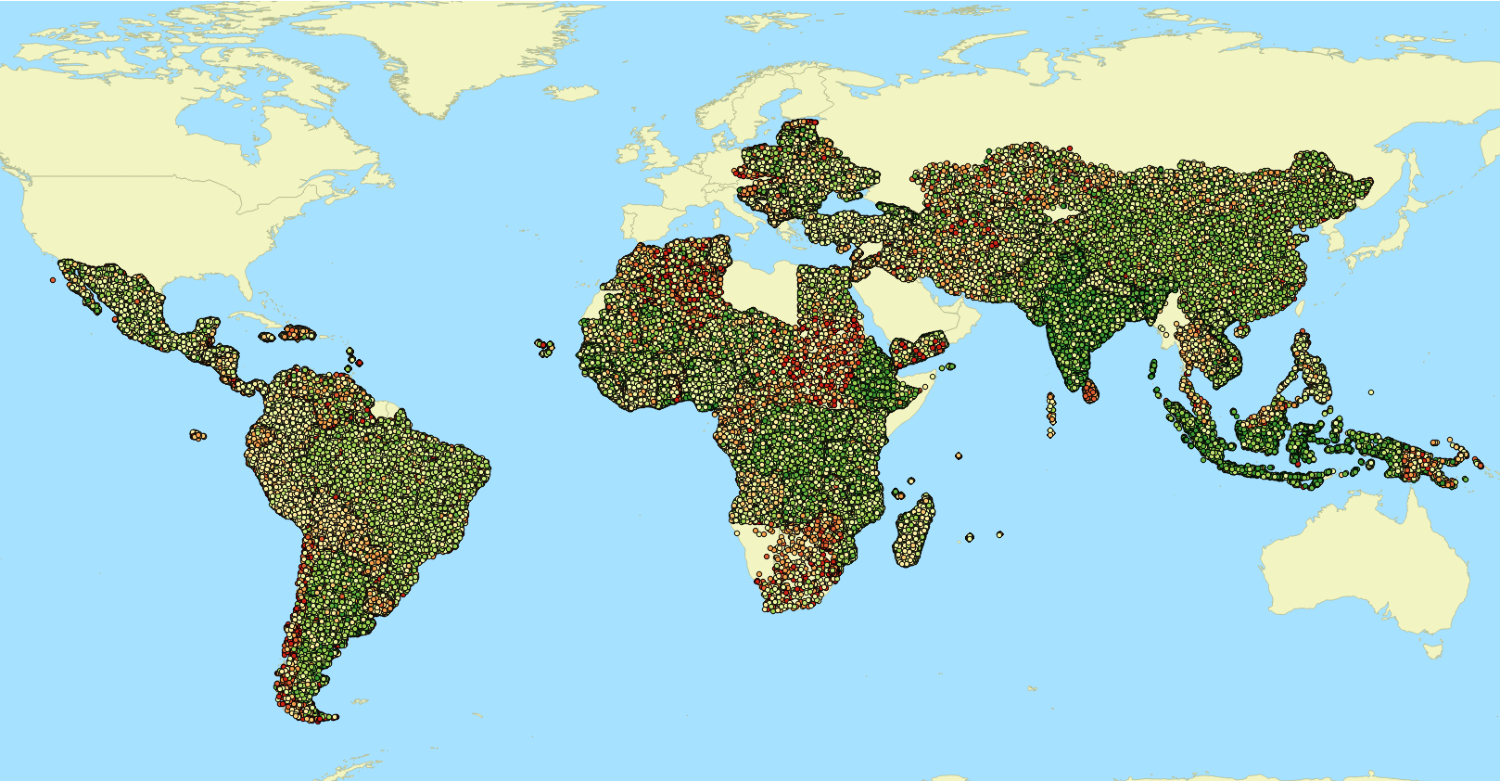
\includegraphics[width=\textwidth,height=1\textheight,keepaspectratio]{../img/risk_map.pdf}
\end{center}
\noindent \footnotesize{\textbf{Source:} Own creation based on \cite{wb_i_map}. \\Data from the World Bank \parencite{wb_data}.}
\end{figure}

